\chapter{Kiến Thức Nền Tảng}
\ifpdf
    \graphicspath{{Chapter2/Chapter2Figs/PNG/}{Chapter2/Chapter2Figs/PDF/}{Chapter2/Chapter2Figs/}}
\else
    \graphicspath{{Chapter2/Chapter2Figs/EPS/}{Chapter2/Chapter2Figs/}}
\fi

\begin{quote}

%Trong chương này, chúng tôi sẽ trình bày những kiến thức nền tảng trên ba chủ đề chính bao gồm\textit{Mạng nơ-ron hồi quy (Recurrent neural network)} và biến thể của nó \textit{Long short-term memory} với khả năng giải quyết vấn đề về các \textit{phụ thuộc dài hạn} (Long term dependencies). Chúng tôi cũng trình bày về mô hình dịch máy nơ-ron dựa trên kiến trúc bộ mã hóa - bộ giải mã đã được đề cập đến trong chương giới thiệu. Những kiến thức được trình bày trong chương này cung cấp những nền tảng cũng như phân tích các vấn đề mà kiến trúc bộ mã hóa - bộ giải mã gặp phải để đi đến chương tiếp theo về cơ chế \textit{Attention} trong dịch máy nơ-ron.

Trong chương này, chúng tôi sẽ trình bày những kiến thức nền tảng trên ba chủ đề bao gồm mạng nơ-ron hồi quy, mô hình ngôn ngữ nơ-ron và mô hình dịch máy nơ-ron. Mạng nơ-ron hồi quy (RNN) là xương sống của dịch máy nơ-ron. Nó được sử dụng để làm cả bộ mã hóa lẫn bộ giải mã. Ứng với mỗi vai trò, RNN sẽ có một thiết kế riêng. Một phiên bản cải tiến của RNN là \textit{Long short-term memory} cũng được chúng tôi trình bày, phiên bản này giúp cho việc huấn luyện RNN trở nên dễ dàng hơn. Sau đó, dựa trên những kiến thức về mạng nơ-ron hồi quy, chúng tôi nói về khái niệm \textit{mô hình ngôn ngữ} với chức năng tạo ra từ trong bộ giải mã, là bước quan trọng trong dịch máy nơ-ron. Cuối cùng, chúng tôi cũng trình bày về mô hình dịch máy nơ-ron theo kiến trúc bộ mã hóa - bộ giải mã với RNN và mô hình ngôn ngữ hồi quy là những thành phần nền tảng.

\end{quote}
\section{Mạng nơ-ron hồi quy (Recurrent neural network)}

Trong tự nhiên, dữ liệu không phải lúc nào cũng được sinh ra một cách ngẫu nhiên. Trong một số trường hợp, chúng được sinh ra theo một thứ tự. Xét trong dữ liệu văn bản, ví dụ ta cần điền vào chỗ trống cho câu sau \textit{Paris là thủ đô của nước \_\_}. Dễ biết được rằng chỉ có duy nhất một từ phù hợp cho chỗ trống này, đó là \textit{Pháp}. Điều này có nghĩa là mỗi từ trong một câu không được tạo ra ngẫu nhiên mà nó được tạo ra dựa trên một liên hệ với những từ đứng trước nó. Các loại dữ liệu khác như những khung hình trong một bộ phim hoặc các đoạn âm thanh trong một bản nhạc cũng có tính chất tương tự. Những loại dữ liệu mang thứ tự này được gọi chung là dữ liệu chuỗi (sequential data).

Trong quá khứ, một số mô hình xử lý dữ liệu chuỗi bằng cách giả định rằng đầu vào hiện tại có liên hệ với một số lượng xác định đầu vào trước đó, ví dụ như giả định Markov. Một cách đơn giản hơn, nhiều mô hình tạo ra một cửa sổ trượt để nối mỗi đầu vào hiện tại với một số lượng đầu vào trước đó nhằm tạo ra sự mô phỏng về tính phụ thuộc. Cách tiếp cận này đã được sử dụng cho mô hình \textit{Deep belief network} trong xử lý tiếng nói \cite{massetal2012}. Nhược điểm của những cách làm này là ta phải xác định trước kích thước của cửa sổ. Một mô hình với kích thước cửa sổ với chiều dài bằng 6 không thể nào quyết định được từ tiếp theo trong câu \textit{Hổ là loài động vật ăn} sẽ là \textit{thịt} hay \textit{cỏ}. Trong ví dụ này, từ tiếp theo của câu phụ thuộc mật thiết vào từ \textit{Hổ} cách nó đúng 6 từ. Trên thực tế, có rất nhiều câu đòi hỏi sự phụ thuộc với nhiều từ xa hơn trước đó. Ta gọi những sự phụ thuộc kiểu như vậy là những \textit{phụ thuộc dài hạn} (long term dependency). 

\textit{Mạng nơ-ron hồi quy} (recurrent neural network) \cite{elman1990} gọi tắt là \textit{RNN} là một nhánh của nạng nơ-ron nhân tạo được thiết kế đặc biệt cho việc mô hình hóa dữ liệu chuỗi. Khác với những mô hình đã đề cập giả định sự phụ thuộc chỉ xảy ra trong một vùng có chiều dài cố định. RNN, trên lý thuyết, có khả năng nắm bắt được các phụ thuộc dài hạn với chiều dài bất kỳ. Để làm được điều đó, trong quá trình học, RNN lưu giữ những thông tin cần thiết cho các phụ thuộc dài hạn bằng một vec-tơ được gọi là \textit{trạng thái ẩn}.

Xét một chuỗi đầu vào $x={x_1,x_2,...,x_n}$. Ta gọi $h_t$ là trạng thái ẩn tại thời điểm $t$, là lúc một mẫu dữ liệu $x_t$ được đưa vào RNN. Trạng thái ẩn $h_t$ không chỉ phụ thuộc vào mẫu dữ liệu hiện tại $x_t$ mà còn dựa trên trạng thái ẩn trước đó $h_{t-1}$. Có thể thể hiện $h_t$ như một hàm hồi quy với tham số là đầu vào hiện tại và chính nó ở thời điểm trước đó:
\begin{equation} \label{basicRnnEquation}
	h_t = f \left(h_{t-1}, x_t \right)
\end{equation}
trong đó hàm $f$ là một ánh xạ phi tuyến. Như vậy, $h_t$ có thể chứa được thông tin của toàn bộ chuỗi đầu vào mà nó đã xử lý nhờ vào định nghĩa đệ quy trong công thức \ref{basicRnnEquation}. Nói một các khác, RNN sử dụng trạng thái ẩn như một dạng bộ nhớ để lưu giữ thông tin từ một chuỗi.

\begin{figure}
	\centering
	\includegraphics[width=0.25\textwidth]{rnn_loop}
	\caption[Mô hình RNN dạng đệ quy]{Mô hình RNN đơn giản với kết nối vòng, \textbf{$h$} được xem như bộ nhớ được luân chuyển trong RNN. Chú ý rằng đường nét đứt ở đầu ra thể hiện rằng tại một thời điểm $t$, RNN có thể có hoặc không có một đầu ra.}
	\label{fig_rnn_loop}
\end{figure}

Hình \ref{fig_rnn_loop} thể hiện định nghĩa hồi quy của RNN, và nó đúng cho chuỗi có độ dài bất kỳ. Tuy nhiên, với một chuỗi có độ dài cố định, RNN có thể được thể hiện dưới dạng \textit{dàn trải ra} (unrolled). Hình \ref{fig_rnn_unrolled} thể hiện dạng dài trải của RNN.

\begin{figure}
	\centering
	\includegraphics[width=0.85\textwidth]{rnn_unrolled}
	\caption[Mô hình RNN dạng dàn trải]{Mô hình RNN được dàn trải (unrolled), ví dụ trong 4 thời điểm.}
	\label{fig_rnn_unrolled}
\end{figure}


Thông thường, hàm $f$ là một hàm phi tuyến như hàm \textit{sigmoid} hay hàm \textit{tanh}. Xét một RNN với công thức cụ thể như sau:
\begin{equation} \label{rnnWithTanh}
	h_t = tanh \left(W_{xh} x_t + W_{hh}h_{t-1} + b_h \right)
\end{equation}

Ở đây $W_{xh}$ là ma trận trọng số kết nối giữa đầu vào và trạng thái ẩn, $W_{hh}$ là ma trận trọng số hồi quy kết nối trạng thái ẩn với chính nó trong các bước thời gian liền kề. Vec-tơ $b_h$ là vec-tơ "bias" của trạng thái ẩn. Tại thời điểm bắt đầu, trạng thái ẩn $h_0$ có thể được khởi tạo bằng 0 hoặc là một vector chứa tri thức có sẵn như trường hợp của bộ giải mã như chúng tôi đã đề cập trong chương 1.

Tại mỗi thời điểm $t$, tùy vào mục tiêu cụ thể của quá trình học mà RNN có thể có thêm một đầu ra $y_t$. Trong ngữ cảnh bài toán dịch máy nơ-ron, đầu ra của RNN trong quá trình giải mã chính là một từ trong ngôn ngữ đích hay nói chung là một đầu ra dạng rời rạc. Với mục tiêu đó, đầu ra dự đoán của RNN $\hat{y}_t$ sẽ có dạng là một phần phối xác suất trên tập các giá trị có thể có ở đầu ra. Phân phối này nhằm dự đoán sự xuất hiện của $\hat{y}_t$.
\begin{equation} \label{rnnOuputSoftmax}
	s_t = W_{hy}h_t + b_y
\end{equation} 
\begin{equation} \label{rnnOuputSoftmaxDistribution}
	\hat{y_t} = softmax(s_t)
\end{equation}

Trong công thức trên, $W_{hy}$, $b_y$ là những tham số gắn với đầu ra của mô hình. $W_{hy}$ là ma trận trọng số kết nối đầu ra, $b_y$ là vec-tơ "bias" ở đầu ra. $s_t$ là một vector có độ dài bằng với là số lượng từ vựng trong ngôn ngữ đích. Vector này được chuẩn hóa thành một phân phối xác suất $\hat{y_t}$ bằng một hàm \textit{softmax}.

Để ý rằng các ma trận trọng số $W_{xh}$, $W_{hh}$, $W_{hy}$ và các vector bias $b_h$, $b_y$ là các tham số học của mô hình và chúng là duy nhất. Có nghĩa là khi những tham số này được học, bất kỳ một đầu vào nào cũng đều sử dụng chung một bộ tham số. Điều này chính là \textit{sự chia sẻ tham số} (parameters sharing) trong mạng nơ-ron hồi quy. Chia sẻ tham số khiến cho mô hình học dễ dàng hơn, nó giúp cho RNN có thể xử lý chuỗi đầu vào với độ dài bất kỳ mà không làm tăng độ phức tạp của mô hình. Quan trọng hơn, nó giúp ích cho việc tổng quát hóa. Đây chính là điểm đặc biệt của RNN so với mạng nơ-ron truyền thẳng.



\subsection{Huấn luyện mạng nơ-ron hồi quy}



\subsection{Long short-term memory}

Hochreiter và Schmidhuber [1997] đã giới thiệu mô hình LSTM chủ yếu ở để khắc phục vấn đề biến mất gradient. Mô hình này tương tự với mô hình 

\section{Mô hình ngôn ngữ}

%Ta hãy xem xét một ví dụ về não người trong quá trình tạo ra các hành động. Khi chạm tay vào vật nóng, não sẽ tạo ra một tín hiệu để ra lệnh cho cơ thể chúng ta rút tay lại. Không những thế, cảm giác nóng sẽ chuyển hóa thành một suy nghĩ. Suy nghĩ này lại được truyền qua não và dựa trên thông tin của giác quan, ta tiếp tục thực hiện một hành động khác. Ví dụ nhúng tay vào nước khi biết có nước gần đó. Có thể hình dung một cách đơn giản rằng não người hoạt động như một hàm \textit{hồi quy}, nó nhận vào thông tin của giác quan và một suy nghĩ nội tại để tạo ra một hành động và suy nghĩ mới. Suy nghĩ mới này bao gồm cả những suy nghĩ trước đó. Cách hoạt động của não người trong ví dụ trên cũng chính là cách mà RNN làm việc. Trong đó, tại mỗi thời điểm, thông tin về giác quan được xem như đầu vào của RNN và đầu ra là một hành động. "Suy nghĩ" hoạt động như một loại bộ nhớ giúp RNN lưu giữ thông tin về bối cảnh, là những gì mà nó đã xử lý trong quá khứ. Việc sở hữu một loại "bộ nhớ" khiến RNN trở thành mô hình phù hợp cho dữ liệu chuỗi.
%Trong thực tế, mạng nơ-ron hồi quy được áp dụng thành công trong các bài toán mô hình hóa ngôn ngữ \cite{mikolovLM}.

%\begin{figure}
%	\centering
%	\includegraphics[width=0.3\textwidth]{rnn_loop}
%	\caption[Mô hình RNN đơn giản]{Mô hình RNN đơn giản}
%	\label{fig_rnn_loop}
%\end{figure}

%Hình \ref{fig_rnn_loop} mô tả cấu trúc cơ bản của RNN. Trong đó $x_t$ và $y_t$ lần lượt là đầu vào và đầu ra của RNN tại thời điểm (time step) $t$. $A$ được gọi là một \textit{tế bào RNN (RNN cell)} , thường là một mạng nơ-ron truyền thẳng. Tại mỗi thời điểm $t$, tế bào RNN sẽ tính toán dựa trên đầu vào $x_t$ và một vector $h$ được gọi là \textit{trạng thái ẩn (hidden state)}, là kết quả của quá trình tính toán tại thời điểm ngay trước đó. Sau khi tính toán, tế bào này tạo ra một trạng thái ẩn mới và trạng thái ẩn này tiếp tục được đưa vào mạng cho những tính toán ở thời điểm sau đó. Quá trình này được thể bằng một vòng lặp trong bản thân tế bào RNN. Lưu ý rằng đường nét đứt bao quanh $x_t$, $y_t$ cho biết đầu vào và đầu ra của tế bào RNN là không bắt buộc.

%\begin{figure}
%	\centering
%	\includegraphics[width=\textwidth]{rnn_unfolded}
%	\caption[Mô hình RNN được giàn trải]{Mô hình RNN được giàn trải}
%	\label{fig_rnn_unfolded}
%\end{figure}

%TODO explain RNN unfolded
%Bên cạnh cách thể hiện kiểu vòng lặp như trên hình \ref{fig_rnn_loop}, RNN còn được thể hiện dưới dạng \textit{dàn trải ra (unfolded)} như trên hình \ref{fig_rnn_unfolded}.


%Một RNN có thể được xem là tổ hợp của các mạng nơ-ron truyền thẳng giống nhau, mỗi mạng dành cho một \textit{thời điểm (time step)}. Ta có thể gọi một mạng nơ-ron truyền thẳng đó là một "tế bào RNN" (RNN cell). Các tế bào này liên kết với nhau dựa trên đầu ra nội tại của chúng gọi là \textit{trạng thái ẩn}, trạng thái ẩn của tế bào đứng trước sẽ được đưa vào tế bào đứng sau và tiếp tục như vậy. Ngoài ra mỗi tế bào có thể nhận đầu vào bên ngoài và tạo ra một đầu ra bên ngoài. Hình \ref{fig_single_rnn_cell} mô tả một tế bào RNN đơn giản và hình \ref{fig_3_rnn_cells} mô tả cách ba tế bào RNN liên kết với nhau. Cách liên kết này được gọi là phiên bản \textit{dàn trải ra (unfolded)} của RNN. Ngoài ra một RNN còn có thể được biểu diễn dưới dạng một tế bào RNN với một liên kết kiểu vòng lặp vào chính bản thân nó (hình \ref{fig_rnn_folded}).

%\begin{figure}
%	\centering
%	\includegraphics[width=\textwidth]{composedrnncells}
%	\caption[Ba tế bào RNN liên kết với nhau]{Ba tế bào RNN liên kết với nhau}
%	\label{fig_3_rnn_cells}
%\end{figure}

%\begin{figure}
%	\centering
%	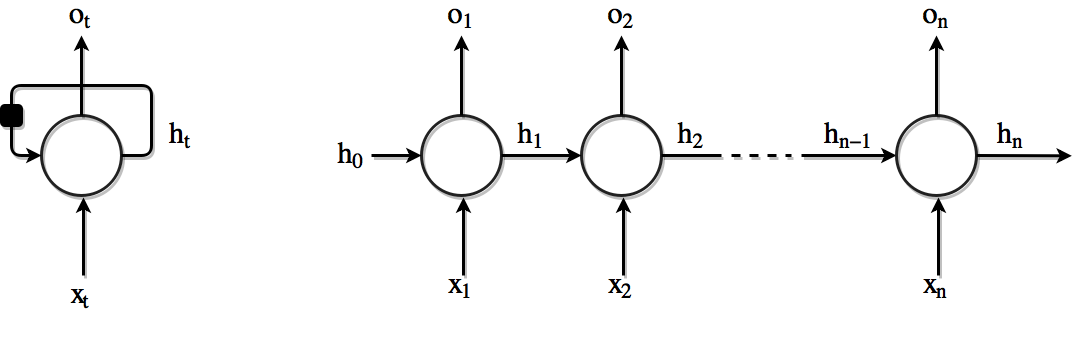
\includegraphics[width=\textwidth]{rnn_folded}
%	\caption[Mạng nơ-ron hồi quy dạng vòng lặp]{Mạng nơ-ron hồi quy dạng vòng lặp}
%	\label{fig_rnn_folded}
%\end{figure}

%Ở dạng dàn trải, một RNN nhận đầu vào là một chuỗi các vector $x_1, x_2,.., x_n$. Tại thời điểm $t (1 \le t \le n)$ vector $x_t$ thuộc chuỗi đầu vào sẽ được đưa vào mạng nơ-ron hồi quy. RNN xử lý vector đó và cập nhật trạng thái ẩn nội tại của nó được đại diện bởi vector $h_t$. Có thể hình dung $h_t$ như là một bộ nhớ lưu giữ thông tin về các vector mà nó đã xử lý cho đến thời điểm $t$. Ở dạng cơ bản nhất, công thức cập nhật trạng thái ẩn của RNN có dạng:



